\section{Receiver Position by Search}
	We describe a search procedure which solves a least-squares problem without forming normal equations. Assume four or more pseudoranges $P_1,P_2,\vdots,P_m$ are given in the same epoch. We want to determine the position of our receiver, with no a priori knowledge of its location.
	
	First we compute the ECEF coordinates of all m satellites from the ephemeris file.Then wc transform the Cartesian coordinates of each satellite at transmission time (which can be obtained from the pseudorange) to $(\varphi_i,\lambda_i)$ = (latitude, longitude). The average of those coordinates is our first guess of the receiver location.
	
	Taking this point as a center we introduce a grid covering a hemisphere. There may be ten equal radial subdivisions out to $\pi/2$ and possibly 16 equal subdivisions of the $2\pi$angle. At each grid point we calculate a residual $R_i=P_i-P_1,i=2,\vdots,m $, as the difference between the observed pseudorange and the first value to eliminate the receiver clock offset. Next we difference these differences:
	\begin{align*}
	 r_1& = R_2-R^0_2 = (P_2-P_1) - (P^0_2-P^0_1) \\
	 r_2& = R_3-R^0_3 = (P_3-P_1) - (P^0_3-P^0_1) \\
	\vdots& \\
	 r_{m-1}& = R_m-R^0_m = (P_m-P_1) - (P^0_m-P^0_1) 
	\end{align*}
	\begin{figure}
		\centering
		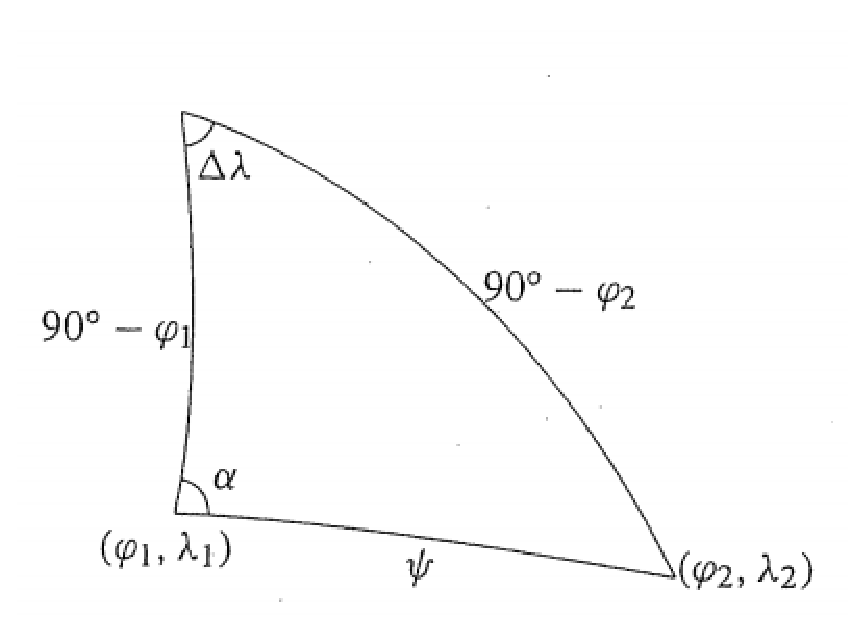
\includegraphics[width=0.7\linewidth]{TeX_files/Part03/chapter09/image/9-15}
		\caption{Spherical triangle for calculation of receiver latitude and longitude $(\varphi,\lambda)$}
		\label{fig:9-15}
	\end{figure}

	This gives a first approximation to the sum $S=\Sigma r^2_i$ Among all the possible values for S , we seek the smallest one; the gridpoint connected to this value is the new guess for the location of the receiver. The grid is made finer for the next iteration. A new gridpoint is determined and selected as center for the following refinement of the grid and
	an subsequent search takes place. The procedure is repeated until no further improvement in position is achieved.
	
	Finally we show how to calculate the new position by spherical trigonometry, as in Figure \ref{fig:9-15}. Let the coordinates of the original point be $(\varphi_1,\lambda_1)$. We want to move $\psi$ degrees along the azimuth a to the new point $(\varphi_2,\lambda_2)$. Computing $\varphi_2$ and $\lambda_2$ is a classical geodetic problem and the following basic equations yield a solution on the sphere:
	\begin{equation}\label{eq:9.32}
		\sin\varphi_2 = \sin\varphi_1\cos\psi+\cos\varphi_1\sin\psi\cos\alpha\quad and \quad \sin\Delta\lambda=\dfrac{\sin\aleph\sin\psi}{\cos\varphi_2}
	\end{equation}
	
	These equations give the latitude $\varphi_2$ of the new point and the increment $\Delta\lambda$ in longitude.The M-file recpos shows a fast implementation of the code. Eventually one finds a receiver position consistent with precision of the orbit, the refraction model, and the pseudoranges.
	
	This is an example of another look at least squares. Here, since $P_1$ is subtracted from every other pseudorange, the differences are obviously correlated. Any error in $P_1$ present in each of the differences. In the search we ignore these correlations since the procedure is designed only to give a first guess of the receiver location.
	
	A least-squares procedure using the proper covariance matrix should follow our search technique. The resulting guess is almost always within the (linear) convergence region. Obtain the navigation data from rinexe(ohiostat.96n,rinex\_n.dat).You may zoom in on the figure by pressing your mouse button. After many zooms you may read off the preliminary position on the x- and y-labeis.
	
	The M-file $get_eph$ opens, reads and reshapes an ephemerides file. Such a file usually contains several data sets for a particular satellite. It is common practice to select the ephemeris that is immediately before the epoch of use. The file $find_eph$ does this. Keeping to this practice, however, eventually leads to a change of ephemeris data. This most probably will introduce a jump in the calculated orbit. More advanced programs smooth orbits, if they have to be exploited over longer periods of time. An even better solution is to change to precise ephemerides.
